\documentclass[%
reprint,
%superscriptaddress,
%groupedaddress,
%unsortedaddress,
%runinaddress,
%frontmatterverbose, 
%preprint,
%preprintnumbers,
nofootinbib,
%nobibnotes,
%bibnotes,
 amsmath,amssymb,
aps,
%pra,
%prb,
%rmp,
%prstab,
%prstper,
%floatfix,
superscriptaddress,
showkeys,
%endfloats,
%onecolumn,
longbibliography
]{revtex4-1}

%TESTE
\usepackage{enumitem}

\usepackage{xr}
\usepackage{tabularx}
\usepackage{booktabs}
\usepackage{graphicx}% Include figure files
\usepackage{dcolumn}% Align table columns on decimal point
\usepackage{bm}% bold math
\usepackage{microtype}
\usepackage{gensymb}
\usepackage{url}
\usepackage[breaklinks, hidelinks, colorlinks=true,linkcolor=blue,citecolor=black]{hyperref}% add hypertext capabilities
\usepackage{color, colortbl}
\usepackage[table,xcdraw]{xcolor}
%\usepackage[mathlines]{lineno}% Enable numbering of text and display math
%\linenumbers\relax % Commence numbering lines

%\usepackage[showframe,%Uncomment any one of the following lines to test 
%%scale=0.7, marginratio={1:1, 2:3}, ignoreall,% default settings
%%text={7in,10in},centering,
%%margin=1.5in,
%%total={6.5in,8.75in}, top=1.2in, left=0.9in, includefoot,
%%height=10in,a5paper,hmargin={3cm,0.8in},
%]{geometry}

%VER
\usepackage[table]{xcolor}

\makeatletter
\renewcommand\frontmatter@abstractwidth{\dimexpr0.9\textwidth\relax}
\makeatother


% \bibliographystyle{apsrev4-1}
\usepackage{algorithm}
\usepackage{algpseudocode}

\makeatletter
\newcommand*{\addFileDependency}[1]{% argument=file name and extension
  \typeout{(#1)}
  \@addtofilelist{#1}
  \IfFileExists{#1}{}{\typeout{No file #1.}}
}
\makeatother

\newcommand*{\myexternaldocument}[1]{%
    \externaldocument{#1}%
    \addFileDependency{#1.tex}%
    \addFileDependency{#1.aux}%
}

\newcommand{\sm}{\scalebox{0.5}[1.0]{\( - \)}}


%VER
\makeatletter
\renewcommand\subparagraph{\@startsection{subparagraph}{5}{\parindent}%
    {3.25ex \@plus1ex \@minus .2ex}%
    {-1em}%
    {\normalfont\normalsize\bfseries}}
\makeatother

\begin{document}

\preprint{1}



\title{VessShape: Few-shot blood vessel segmentation by leveraging shape priors from synthetic images}
%VessShape: Few-shot blood vessel segmentation using shape priors from synthetic data
%VessShape: Adding shape priors to neural networks for few-shot blood vessel segmentation

\author{Wesley Nogueira Galvão}
\affiliation{Department of Computer Science, Federal University of S\~ao Carlos, S\~ao Carlos, SP, Brazil}


\author{Cesar H. Comin}
\email[Corresponding author: ]{comin@ufscar.br}
\affiliation{Department of Computer Science, Federal University of S\~ao Carlos, S\~ao Carlos, SP, Brazil}

\date{\today}% It is always \today, today,
             %  but any date may be explicitly specified

\begin{abstract}

??

\end{abstract}

\keywords{Blood vessel segmentation, Connectivity, post-processing}

\maketitle
\thispagestyle{plain}
%\ohead*{\pagemark}

\section{Introduction}
\label{sec:introduction}



\section{Related Works}
\label{sec:related}

- Pre-training with synthetic data

- Synthetic data in medical images

- Shape priors for medical images segmentation using neural networks

- Shape priors for vessel segmentation (classic methods)

- Shape priors for vessel segmentation (neural networks)

\section{Methodology}
\label{s:methodology}

\subsection{VessShape Dataset}

VessShape is a synthetic image dataset that combines tubular, vessel-like shapes with diverse foreground and background textures. The central idea is to provide a robust set that can be used to train blood vessel segmentation models while keeping geometric priors fixed and drastically changing texture, encouraging models to learn shape cues (connectivity, tapering, bifurcations) rather than overfitting to texture.

The geometry of this dataset is based on Bézier curves, which allow a flexible and controlled representation of tubular shapes. Each vascular branch $C_k$ is described by an $n$-th order Bézier curve with control points $\{\mathbf{P}_{k,i}\}_{i=0}^n$, sampled to produce connected branches and plausible bifurcation angles. Tortuosity is adjusted by small perturbations to the control points, ensuring that vessel geometry is realistic and diverse. The Equation \ref{eq:bezier} defines the Bézier curve $\mathbf{c}_k(t)$ for each branch $k$, where $t$ varies from 0 to 1.

\begin{equation}
\mathbf{c}_k(t) \,=\, \sum_{i=0}^{n} \binom{n}{i} (1-t)^{n-i} t^{i} \, \mathbf{P}_{k,i}, \qquad t \in [0,1].
\label{eq:bezier}
\end{equation}

To generate connected vascular trees, control points are sampled so that branches share endpoints in order to form plausible bifurcation angles. Tortuosity is induced by random perturbations to the control points, with amplitude regulated by the displacement scale $\delta$. The number of branches $K$ and the order $n+1$ of the Bézier curves are also randomly sampled to ensure a wide variety of shapes, and the radius $r_0$ sets the basal thickness of the vessels during the rasterization process. Table \ref{tab:vessshape_params} summarizes the parameters used in the VessShape dataset generation, along with their sampling ranges and descriptions.

\begin{table*}[t]
\caption{VessShape generation parameters, sampling ranges, and description.}
\label{tab:vessshape_params}
\centering
\begin{tabularx}{\textwidth}{l c X}
\hline
    \textbf{Parameter} & \textbf{Range} & \textbf{Description} \\
\hline
Number of curves $K$ & $[1,20]$ & Number of branches/vessels generated per sample. \\
Control points $n{+}1$ & $[2,20]$ & Bézier curve complexity (order $n$). \\
Displacement scale $\delta$ (px) & $[50.0,150.0]$ & Controls curvature/tortuosity via the typical amplitude of control-point displacement. \\
Initial radius $r_{0,k}$ (px) & $[1,5]$ & Basal vessel thickness; a smooth taper is applied along the branch. \\
Matting blur $\sigma$ & $[1,2]$ & Standard deviation of the Gaussian used for $A = G_{\sigma} * M$. \\

\hline
\end{tabularx}
\end{table*}


The generation of the binary mask $M$ from the curves $\mathbf{c}_k(t)$ is a multi-step process. Initially, each curve is discretized by sampling points at a sufficient resolution to capture its curvature, which are then sequentially connected to form a 1-pixel-thick polyline on the image grid. Subsequently, a binary morphological dilation with a disk-shaped structuring element is applied iteratively until the structure reaches a radius of $r_0$, consequently assigning a constant tubular thickness to the branches. Optionally, a morphological closing operation can be employed to seal small gaps at bifurcations or sharp angles.

To compose the final image $I$ from a binary mask $M$, a foreground texture $F$ and a background texture $B$ are selected from distinct categories, randomly cropped, and resized to the target dimensions ($H \times W$). An alpha matte $A$ is then generated by smoothing $M$ with a Gaussian filter of standard deviation $\sigma$ and normalizing its values to the $[0, 1]$ range. The textures are subsequently blended using this matte according to Eq.~\ref{eq:compose}, which ensures that vessel regions ($A \approx 1$) preserve the foreground while non-vessel regions ($A \approx 0$) retain the background. The parameter $\sigma$ directly controls the smoothness of this transition at the vessel boundaries. After composition, the image $I$ undergoes channel-wise normalization using ImageNet statistics for compatibility with pre-trained models. Finally, to ensure spatial consistency, any geometric augmentations are applied identically to both the image $I$ and its corresponding mask $M$. A sample of the generated images and masks is shown in Figure \ref{f:vess-shape_sample}.

\begin{equation}
I(x) \,=\, A(x)\,F(x) + (1-A(x))\,B(x), \qquad x \in \Omega.
\label{eq:compose}
\end{equation}


\begin{figure*}[tbp]
    \centering
    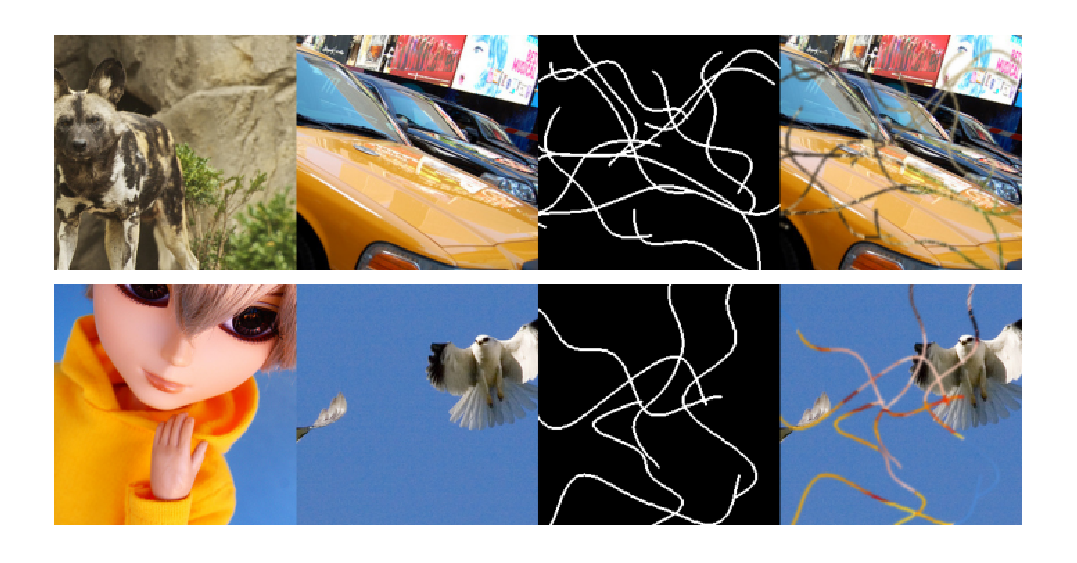
\includegraphics[width=\textwidth]{figures/results/vess-shape_sample.pdf}
    \caption{??.}
    \label{f:vess-shape_sample}
\end{figure*}


\subsection{Training details}

A crucial step is the choice of architecture. We adopt an encoder–decoder arrangement, in which the encoder extracts visual representations and the decoder performs the segmentation. In the encoder, the architectures actually evaluated were ResNet18 and ResNet50 \cite{}. The decoder follows the U-Net design \cite{}, widely used in medical segmentation.

We design three complementary stages with distinct goals: (i) pretraining on VessShape to inject a \emph{shape} bias and reduce dependence on texture, (ii) \emph{from scratch} training on natural datasets (VessMAP, DRIVE) to establish a baseline, and (iii) \emph{few-shot} fine-tuning to measure the transferability and sample efficiency of the learned representations.

\subsection{Pre-training on VessShape}




\subsection{Fine-tuning}

- Datasets (VessMAP e DRIVE)

- Procedure

\section{Results}
\label{s:results}

\begin{figure*}[tbp]
    \centering
    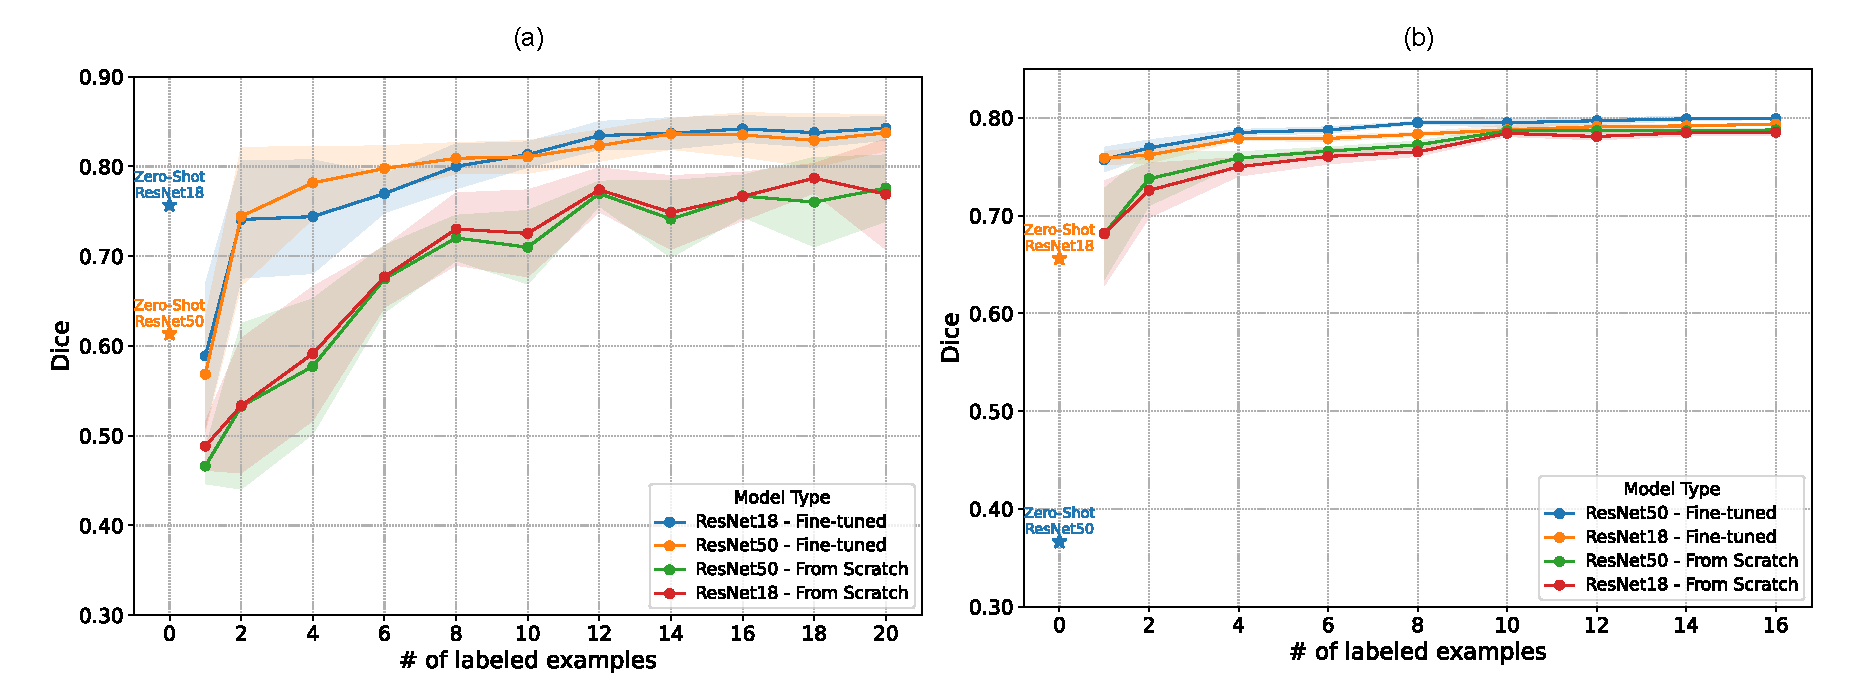
\includegraphics[width=\textwidth]{figures/results/results_charts.pdf}
    \caption{??.}
    \label{f:results_charts}
\end{figure*}


\begin{table*}[t]
\caption{Zero-shot segmentation results.}
\label{tab:zero_shot_results}
\centering
\begingroup
\small
\setlength{\tabcolsep}{3pt}
\renewcommand{\arraystretch}{1.15}
\begin{tabularx}{\textwidth}{l X r r r r r r}
\hline
	\textbf{Dataset} & \textbf{Model} & \textbf{Acc} & \textbf{IoU} & \textbf{Prec} & \textbf{Rec} & \textbf{Dice} & \textbf{AUC} \\
\hline
VessMAP & ResNet18 - From Scratch & 0.886 & 0.616 & 0.846 & 0.696 & 0.757 & 0.932 \\
VessMAP & ResNet50 - From Scratch & 0.817 & 0.472 & 0.746 & 0.605 & 0.614 & 0.854 \\
\hline
DRIVE & ResNet18 - From Scratch & 0.907 & 0.490 & 0.629 & 0.699 & 0.656 & 0.891 \\
DRIVE & ResNet50 - From Scratch & 0.888 & 0.230 & 0.728 & 0.275 & 0.367 & 0.762 \\
\hline
\end{tabularx}
\endgroup
\end{table*}


\section{Conclusion}
\label{s:conclusion}




\section*{Funding}
C. H. Comin thanks FAPESP (grant no. 21/12354-8) for financial support. 


\bibliography{references}

\end{document}